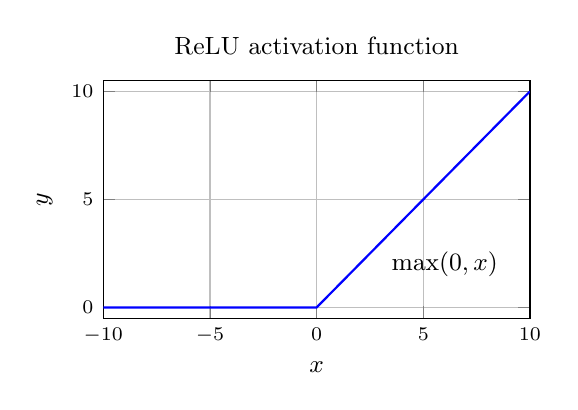
\begin{tikzpicture}
\begin{axis}[width=7cm, height=4.6cm, grid=both, xmin=-10, xmax=10, ymin=-0.5, ymax=10.5,
  xlabel={$x$}, ylabel={$y$}, title={ReLU activation function}, title style={font=\small},
  tick label style={font=\scriptsize}, label style={font=\small}]
\addplot[blue, thick, domain=-10:10, samples=3] {max(0,x)};
\node[font=\small] at (axis cs:6,2) {$\max(0,x)$};
\end{axis}
\end{tikzpicture}
